\documentclass{article}

\usepackage[utf8]{inputenc} 
\usepackage[russian]{babel}
\usepackage{amsmath,amssymb}
\usepackage{tipa}
\usepackage{hyperref}
\usepackage{graphicx}
\usepackage{comment}
\usepackage{fancyhdr}
\usepackage[tocflat]{tocstyle}
\usepackage{titlesec}
\binoppenalty=10000
\relpenalty=10000
\usepackage{multicol}
\usepackage[left=2cm,right=2cm,
    top=2cm,bottom=2cm,bindingoffset=0cm]{geometry}
\usepackage{xcolor}
\definecolor{linkcolor}{HTML}{2832C2} % цвет ссылок
\definecolor{urlcolor}{HTML}{2832C2} % цвет гиперссылок
\hypersetup{pdfstartview=FitH,  linkcolor=linkcolor,urlcolor=urlcolor, colorlinks=true}
\setlength{\parindent}{5ex}
    
\titleformat{\section}[block]{\Large\bfseries\filcenter}{}{1em}{}

\makeatletter
\renewcommand\tableofcontents{%
  \null\hfill\textbf{\Large\contentsname}\hfill\null\par
  \@mkboth{\MakeUppercase\contentsname}{\MakeUppercase\contentsname}%
  \@starttoc{toc}%
}
\makeatother
    
\title{\textbf{Дифференциальные уравнения\\ Билеты}}
\author{DK3!8}

\begin{document}

  \pagenumbering{gobble} 
  \maketitle
  \pagenumbering{arabic}

\tableofcontents
\newpage

\section{Билет №1. Уравнение с разделяющимися переменными: общее решение, общая схема
исследования}
\textbf{Определение.} Уравнение в дифференциалах вида.
\begin{equation}
  X(x)dx + Y(y)dy = 0 \label{formula1}
\end{equation}
называют \textbf{уравнением с разделенными переменными.}\\
\\
\textbf{Теорема (общее решение УРП).} Пусть $X \in C(a,b)$, $Y \in C(c,d)$, $(\alpha, \beta) \subset (a,b)$. Тогда
\begin{enumerate}
    \item если $y$ --- решение на $(\alpha, \beta)$ уравнения (\ref{formula1}), то при некотором значении $C \in \mathbb{R}$ функция $y$ неявно задается уравнением
    \begin{equation}
        \int X(x)dx + \int Y(y)dy = C \label{formula2}
    \end{equation}
    \item если при некотором значении $C \in \mathbb{R}$ уравнение (\ref{formula2}) неявно задает функцию $y \in C^1(\alpha, \beta)$, то $y$ --- решение уравнения (\ref{formula1}) на $(\alpha, \beta)$. 
\end{enumerate}
\textbf{Доказательство}
\begin{enumerate}
    \item Покажем, что функция $y(x)$ удовлетворяет уравнению (\ref{formula2}) при любом $x \in (\alpha, \beta)$ и некотором $C \in \mathbb{R}$. Имеем
    \begin{equation*}
        \int X(x)dx + \int Y(y)dy = \int X(x)dx + \int Y(y)y'dx = \int (X(x) + Y(y)y')dx
    \end{equation*}
    Так как $y$ --- решение уравнения (\ref{formula1}) на $(\alpha, \beta)$, то $\forall x \in (\alpha, \beta)$ подынтегральное выражение равно нулю $\implies$ интеграл равен некоторой постоянной.
    \item Покажем, что функция $y(x)$ удовлетворяет уравнению (\ref{formula1}) $\forall x \in (\alpha, \beta)$. Дифференцируя обе части (\ref{formula2}), получим
    \begin{equation*}
        X(x) + Y(y)y' = 0
    \end{equation*}
    Исходя из условия, это равенство выполнено тождественно на $(\alpha, \beta)$ $\implies$ $y$ --- решение уравнения (\ref{formula1}) по определению.
\end{enumerate}
\\
\textbf{Определение.} Уравнение вида
\begin{equation}
    p_1(x)q_1(y)dx + p_2(x)q_2(y)dy = 0 \label{formula3}
\end{equation}
называют \textbf{уравнением с разделающимися переменными}.\\

При делении на $q_1(y)p_2(x)$ уравнение приводится к уравнению с разделенными переменными. Необходимо убедиться, что не происходит деления на ноль.

Пусть $p_1, p_2 \in C(a,b)$ и $q_1, q_2 \in C(c,d)$. Если $q_1(y_0) = 0$, то $y \equiv y_0$, $x \in (a,b)$ --- решение исходного уравнения. Для поиска других интегральных кривых требуется разбить область задания уравнения на две подобласти, общей границей которых является прямая $y = y_0$.

Аналогично следует поступить для $p_2(x_0) = 0$. В таком случае $x \equiv x_0$, $y \in (c,d)$ --- решение исходного уравнения.

Разбив всю область на необходимое количество частей, нужно рассмотреть исходное уравнение на каждой части отдельно. На каждой такой подобласти можно разделить исходное уравнение на $q_1(y)p_2(x)$, не опасаясь получить ноль в знаменателе.

Изучив поведение интегральных кривых вблизи границ, делается вывод о наличии особых и составных решений уравнения на исходной области его задания.\\

\textbf{Теорема (существование и единственность решения задачи Коши для УРП)}. Пусть $X \in C(a,b)$, $Y \in C(c,d)$, $(x_0, y_0)$ --- не особая точка уравнения (\ref{formula1}). Тогда в некоторой окрестности точки $(x_0, y_0)$ уравнение
\begin{equation*}
    \int_{x_0}^{x} X(s)ds + \int_{y_0}^{y} Y(s)ds = 0
\end{equation*}
определяет единственную интегральную кривую уравнения (\ref{formula1}), проходящую через точку $(x_0, y_0)$.

\section{Билет №2. Линейное уравнение 1-го порядка: общее решение ЛОУ, общее решение
ЛНУ. Метод Лагранжа и метод интегрирующего множителя.}
\textbf{Определение.} Дифференциальное уравнение вида
\begin{equation}
    y' = p(x)y + q(x) \label{lnu}
\end{equation}
называется \textbf{линейным уравнением первого порядка.}\\

\noindent \textbf{Определение.} Уравнение (\ref{lnu}) называется \textbf{однородным}, если $q \equiv 0$ на $(a,b)$, иначе \textbf{неоднородным}.\\

\hypertarget{loulemma}
\noindent \textbf{Лемма (общее решение ЛОУ 1-го порядка).} Пусть $p \in C(a,b)$. Тогда общее решение уравнения
\begin{equation}
    y' = p(x)y \label{lou}
\end{equation}
имеет вид
\begin{equation*}
    y = Ce^{\int p},\quad dom\,y = (a,b), \quad C \in \mathbb{R}
\end{equation*}
\noindent \textbf{Доказательство.} Заметим, что функция, тождественно равная нулю на $(a,b)$, является решением. По теореме о единественности решения ЗК оно не является особым. В области, где $y > 0$, исходное уравнение равносильно
\begin{equation*}
    \frac{dy}{y} = p(x)dx
\end{equation*}
Интегрируя, получаем
\begin{equation*}
    \ln y = \int p(x)dx + C
\end{equation*}
Отсюда
\begin{equation*}
    y = Ae^{\int p(x)dx},\, A > 0
\end{equation*}
По теореме об общем решении УРП полученное соотношение описывает все интегральные кривые в области, где $y > 0$.

Аналогично с $y < 0$. Таким образом, все решения имеют требуемый вид.\\

\noindent \textbf{Теорема (Общее решение ЛУ 1-го порядка).} Пусть $p,q \in C(a,b)$. Тогда общее решение уравнения (\ref{lnu}) имеет вид
\begin{equation}
    y = (C + \int qe^{-\int p})e^{\int p} \label{lnusol}
\end{equation}
\textbf{Доказательство.} Подстановкой легко убеждаемся, что указанная функция при любом $C$ является решением на $(a,b)$.

Проверим, что нет других решений. Докажем от противного. Пусть имеется решение $\varphi$ на $(\alpha, \beta) \subset (a,b)$, не определяемое формулой (\ref{lnusol}) ни при каком $C$. Пусть еще $x_0 \in (\alpha, \beta)$, $\varphi(x_0) = y_0$. При
\begin{equation*}
    C = \left[y_0e^{-\int p(x)dx} - \int q(x)e^{-\int p(x)dx}dx\right]_{x=x_0}
\end{equation*}
функция определена на $(\alpha, \beta)$ и является решением ЗК для уравнения (\ref{lnu}) с начальным условием $y(x_0) = y_0$. Тогда $y \equiv \varphi$ на $(\alpha, \beta)$ по теореме о единственности решения ЗК, что противоречит предположению о функции $\varphi$.

Существует также \textbf{метод Лагранжа}, который позволяет решить уравнение (\ref{lnu}). Он состоит в следующем. По \hyperlink{loulemma}{лемме} решение соответсвующего однородного уравнения имеет вид
\begin{equation}
    y = Ce^{\int p} \label{lousol2}
\end{equation}
где $C$ --- произвольная постоянная. Это выражение подставляют в исходное уравнение (\ref{lnu}), при этом считая $C$ функцией от $x$. Получается уравнение относительно функции $C$:
\begin{equation*}
    C' = qe^{-\int p}
\end{equation*}
Его решение совпадает с выражением в скобках в (\ref{lnusol}). Поэтому общее решение исходного уравнения (\ref{lnu}) получится, если найденную функцию $C$ подставить вместо постоянной $C$ в общем решении (\ref{lousol2}) однородного уравнения.

\section{Билет №3. Равностепенно непрерывные функции. Лемма Арцела–Асколи.}
\textbf{Определение.} Множество функций $F = \{f\}$, определенных на $D$, называется \textbf{равностепенно непрерывным} на $D$, если $\forall \varepsilon > 0$ $\exists \delta > 0$, такое что $\forall f \in F$ и $\forall x_1, x_2 \in D$ из неравенства $|x_2 - x_1| < \delta$ $\implies$ $|f(x_2) - f(x_1)| < \varepsilon$.\\

\noindent \textbf{Лемма (Арцела-Асколи).} Пусть функции последовательности $\{f_n\}_{n=1}^{\infty}$ равномерно ограничены и равностепенно непрерывны на $[a,b]$. Тогда из нее можно выделить подпоследовательность, равномерно сходящуюся на $[a,b]$.\\
\noindent \textbf{Доказательство.} По условию
\begin{equation*}
    M = \sup_{n \in \mathbb{N}, x \in [a,b]} |f_n(x)| < +\infty
\end{equation*}
Составим последовательность чисел
\begin{equation*}
    \varepsilon_k = \frac{M}{2^{k+1}}, \quad k \in \mathbb{N}
\end{equation*}

В силу равностепенной непрерывности последовательности, по каждому $\varepsilon_k$ можно подобрать $\delta_k$, такое что если $x_1, x_2 \in [a,b]$ и $|x_2 - x_1| < \delta_k$, то для любого $n$ будет $|f_n(x_2) - f_n(x_1)| < \varepsilon_k$.

График каждой функции $f_n$ расположен в прямоугольнике $[a,b] \times [-M, M]$. Разобьем этот прямоугольник на меньшие прямоугольники с вертикальной стороной $\varepsilon_1$ и горизонтальной стороной, не превосходящей $\delta_1$ (см. \hyperref[squares]{рисунок}).

\begin{figure}[h!]\label{squares}
    \center{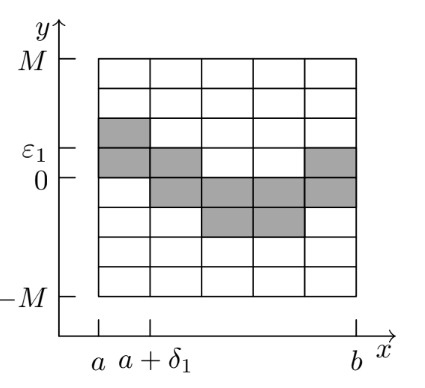
\includegraphics[scale=0.5]{Pics/Screenshot from 2021-01-14 20-32-54.png}}
\end{figure}

График каждой фукнции $f_n$ проходит не более, чем по двум соседним прямоугольникам каждой вертикальной полосы. Количество смежных пар прямоугольников в первой полосе конечно. Значит, найдется пара, по которой проходит бесконечное множество графиков функции последовательности --- закрасим ее. Будем рассматривать теперь только те функции, графики которых проходят по закрашенным прямоугольникам. Во второй полосе выберем пару соседних прямоугольников, через которые проходит бесконечное множество функций из выбранного семейства. Эту пару также закрасим и далее будем рассматривать только те функции, графики которых проходят по закрашенной области.

За конечное число шагов доберемся до крайней правой полосы. Таким образом, получим множество (закрашено на \hyperref[squares]{рисунке}), внутри которого проходят графики функций некоторой последовательности $F_1^{*} = \{f_{n_k}\}$. Для любых функций $f, g \in F_1^{*}$ верно: $|f(x) - g(x)| < 2\varepsilon_1$ при любом $x \in [a,b]$.

Выберем первую функцию из $F_1^{*}$ и обозначим ее $f_1^{*}$. Проведем те же рассуждения для оставшейся последовательности. Получим последовательность $\{f_n^{*}\}$.

По критерию Коши докажем, что последовательность $\{f_n^{*}\}$ сходится равномерно на $[a,b]$.

Зафиксируем $\varepsilon > 0$. Найдем такое $N$, что $2\varepsilon_N < \varepsilon$. При любом $k \in \mathbb{N}$ будет $f_N^*, f_{N+k}^* \in F_N^*$, поэтому при любом $x \in [a,b]$
\begin{equation*}
    |f_N^*(x) - f_{N + k}^*(x)| < 2\varepsilon_N < \varepsilon
\end{equation*}
Таким образом, последовательность $\{f_n^*\}$ сходится равномерно.

\section{Билет №4. ЗК для нормальной системы. Лемма о равносильном интегральном уравнении. Лемма: свойства ломаной Эйлера, определённой на отрезке Пеано.}
\textbf{Определение.} \textbf{Нормальной системой} дифференциальных уравнений порядка $n$ называется система уравнений вида
\begin{equation*}
    \begin{cases}
    \dot{x}_1 = f_1(t, x_1,...,x_n)\\
    ...\\
    \dot{x}_n = f_n(t, x_1, ..., x_n)
    \end{cases}
\end{equation*}

Если ввести в рассмотрение векторы
\begin{equation*}
    r = \begin{pmatrix}
    x_1\\
    ...\\
    x_n
    \end{pmatrix}, \quad
    f(t,r) = \begin{pmatrix}
        f_1(t,r)\\
        ...\\
        f_n(t,r)
    \end{pmatrix}
\end{equation*}
то систему можно компактно записать в виде одного $n$-мерного уравнения
\begin{equation}
    \dot{r} = f(t,r) \label{normsyst}
\end{equation}

\noindent \textbf{Определение.} Вектор-функция $\varphi$ --- \textbf{решение системы} (\ref{normsyst}), если
\begin{itemize}
    \item $\varphi \in C^1((a,b) \to \mathbb{R}^n)$
    \item $\dot{\varphi}(t) \equiv f(t, \varphi(t))$ на $(a,b)$
\end{itemize}

\noindent \textbf{Определение.} \textbf{Задачей Коши} для системы (\ref{normsyst}) называется задача нахождения ее решения, удовлетворяющего начальному условию $r(t_0) = r_0$.\\

\noindent \textbf{Лемма (О равносильном интегральном уравнении.)} Пусть $t_0 \in [a,b]$, $G \subset \mathbb{R}^{n + 1}$ --- область, $(t_0, r_0) \in G$, $f \in C(G \to \mathbb{R}^n)$. Тогда $\varphi$ --- решение на $[a,b]$ задачи Коши.
\begin{equation}
    \dot{r} = f(t,r), \quad r(t_0)=r_0 \label{zksyst}
\end{equation}
если и только если $\varphi$ --- решение на $[a,b]$ уравнения
\begin{equation}
    r(t) = r_0 + \int_{t_0}^{t} f(\tau, r(\tau))d\tau \label{inteq}
\end{equation}
\textbf{Доказательство.} Пусть $\varphi$ --- решение (\ref{zksyst}) на $[a,b]$. Тогда $\varphi \in C[a,b]$. Интегрируя равенство $\dot{\varphi}(\tau) = f(\tau, \varphi(\tau))$ от $t_0$ до $t \in [a,b]$, имеем
\begin{equation*}
    \varphi(t) - \varphi(t_0) = \int_{t_0}^{t} f(\tau, \varphi(\tau))d\tau
\end{equation*}
Поскольку $\varphi(t_0) = r_0$, то функция $\varphi$ --- решение уравнения (\ref{inteq}) по определению.

Докажем обратное. Пусть $\varphi$ --- решение (\ref{inteq}) на $[a,b]$. Тогда из равенства
\begin{equation}
    \varphi(t) = r_0 + \int_{t_0}^{t} f(\tau, r(\tau))d\tau \label{phieq}
\end{equation}
следует, что $\varphi \in C^1[a,b]$. Дифференцируя (\ref{phieq}) по $t$, получаем $\dot{\varphi} \equiv f(t, \varphi(t))$ на $[a,b]$. Кроме того, из (\ref{phieq}) вытекает $\varphi(t_0) = r_0$. Таким образом, $\varphi$ --- решение (\ref{zksyst}) по определению.\\

\noindent \textbf{Определение.} Пусть $G \subset \mathbb{R}_{t,r}^{n+1}$ --- область, $(t_0, r_0) \in G$. Поскольку $G$ --- открытое множество, то найдутся числа $a,b > 0$, такие что параллелепипед
\begin{equation*}
    \Pi = \left\{(t,r) \in \mathbb{R}^{n+1}\,|\, |t-t_0| \le a, |r-r_0|\le b \right\}
\end{equation*}
целиком содержится в области $G$. Так как $\Pi$ --- компакт, то существует число $M = \displaystyle\max_{(t,r)\in \Pi} |f(t,r)|$. Положим $h = \min \{a, \frac{b}{M}\}$ (если $M = 0$, то $h = a$). Отрезок $[t_0 - h, t_0 + h]$ называется \textbf{отрезком Пеано}, соответсвующим точке $(t_0, r_0)$ (см. \hyperref[peano]{рисунок}).

Отрезок Пеано, таким образом, определен неоднозначно. Зафиксируем один из них и разобъем его правую половину на $N \in \mathbb{N}$ равных частей точками
\begin{equation*}
    t_k = t_0 + \frac{kh}{N}, \quad k \in [1 : N]
\end{equation*}
Определим ломаную Эйлера $E_N$: $[t_0, t_0 + h] \to \mathbb{R}$ рекуррентно:
\begin{equation}
    \begin{aligned}
        &E_N(t_0) = r_0,\\
        &E_N(t) = E_N(t_k) + f(t_k, E_N(t_k))(t - t_k), \text{ если } t \in (t_k, t_{k+1}]
        \label{eulerlom}
    \end{aligned}
\end{equation}

Если $(t_k, E_N(t_k)) \notin G$ при некотором $k$, то функция $E_N$ не может быть определена на всем промежутке $[t_0, t_0 + h]$. Следующая лемма показывает, что такая ситуация исключена.\\

\noindent \textbf{Лемма (свойства ломаной Эйлера).} Для любого $t \in [t_0, t_0 + h]$
\begin{enumerate}
    \item функция $E_N$ определена в точке $t$
    \item $|E_N(t) - r_0| \le M(t - t_0)$
\end{enumerate}
\textbf{Доказательство.} Методом математической индукции установим, что утверждения (1) и (2) верны при $t \in [t_0, t_k]$ для любого $k \in [1 : N]$.

При $k = 1$ функция $E_N$ определена на $[t_0, t_1]$. Имеем
\begin{equation*}
    |E_N(t) - r_0| = |r_0 + f(t_0, r_0)(t - t_0) - r_0| = |f(t_0, r_0)|(t - t_0) \le M(t - t_0)
\end{equation*}
\begin{figure}[h!]\label{peano}
    \center{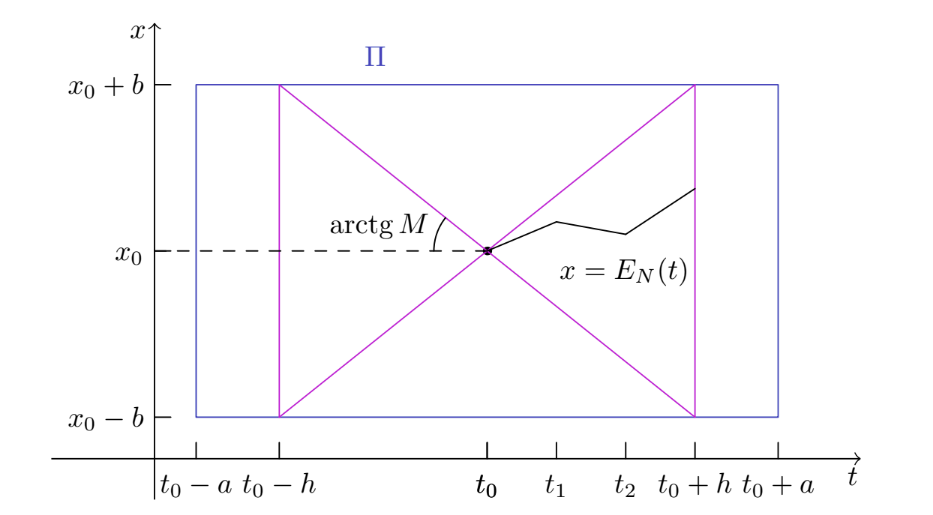
\includegraphics[scale=0.5]{Pics/Screenshot from 2021-01-14 22-03-34.png}}
\end{figure}

Допустим, что утверждения (1) и (2) установлены для $t \in [t_0, t_k]$ при некотором $k \in [1 : N - 1]$. Из пункта (2) тогда следует
\begin{equation*}
    |E_N(t_k) - r_0| \le M(t_k - t_0) \le Mh \le M \frac{b}{M} = b
\end{equation*}
то есть $(t_k, E_N(t_k)) \in \Pi$, а значит $E_N$ можно определить на $[t_k, t_{k+1}]$.

Проверим (2) при $t \in (t_k, t_{k+1}]$:
\begin{equation*}
    \begin{aligned}
        &|E_N(t) - E_N(t_0)| \le |E_N(t) - E_N(t_k)| + |E_N(t_k) - E_N(t_0)| \le\\
        &\le |f(t_k, E_N(t_k))|(t-t_k) + M(t_k - t_0) \le M(t - t_k) + M(t_k - t_0) = M(t - t_0)
    \end{aligned}
\end{equation*}

\section{Билет №5. Теорема Пеано о существовании решения ЗК.}
\textbf{Теорема.} Пусть $G \subset \mathbb{R}_{t,r}^{n + 1}$ --- область, $f \in C(G \to \mathbb{R}^n)$, $(t_0, r_0) \in G$. Тогда задача
\begin{equation*}
    \dot{r} = f(t,r), \quad r(t_0) = r_0
\end{equation*}
имеет решение, определенное на отрезке Пеано, соответствующему $(t_0, r_0)$\\
\textbf{Доказательство.} Не умаляя общности считаем, что $t_0 = 0$, $r_0 = 0$ (в противном случае перенесем начало координат в точку $(t_0, r_0)$).

Пусть $[-h, h]$ --- отрезок Пеано, соответсвующий начальной точке. Установим существование решения на $[0, h]$. Существование решения на $[-h, 0]$ тогда получится как следствие, если в исходном уравнении заменить $t$ на $-t$. Объединяя решения на $[-h, 0]$ и $[0, h]$, по лемме о гладкой стыковке решений получим решение на $[-h, h]$.

Построим последовательность ломаных Эйлера $\{E_N\}_{N=1}^{\infty}$. По свойствам ломаной Эйлера $|E_N(t)| \le Mh \le b$. Значит, последовательность $\{E_N\}$ равномерно ограничена.

Пусть $\varepsilon > 0$, $\delta = \frac{\varepsilon}{M}$. При $t_1, t_2 \in [0, h]$, $t_1 < t_2$, $|t_2 - t_1| < \delta$. По формуле Ньютона- Лейбница находим
\begin{equation*}
    |E_N(t_2) - E_N(t_1)| = \left|\int_{t_1}^{t_2} \dot{E}_N(\tau)d\tau\right| \le \int_{t_1}^{t_2} \dot{E}_N(\tau)d\tau
\end{equation*}
Из определения ломаной Эйлера следует, что $|\dot{E}_N| \le M$ в точках, где производная определена. Тогда
\begin{equation*}
    |E_N(t_2) - E_N(t_1)| \le M(t_2 - t_1) < M\delta = \varepsilon
\end{equation*}
значит, последовательность $\{E_N\}$ равностепенно непрерывна.

По лемме Арцела-Асколи найдется подпоследовательность $\{E_{N_m}\}$, равномерно сходящаяся к некоторой функции $\varphi \in C([0,h] \to \mathbb{R}^n)$. Покажем, что $\varphi$ --- это и есть решение поставленной ЗК.

В силу леммы о равносильном интегральном уравнении достаточно установить, что для $\varphi$ верно
\begin{equation*}
    \varphi(t) \equiv \int_{0}^{t} f(\tau, \varphi(\tau))d\tau \quad \text{на } [0,h]
\end{equation*}
Не умаляя общности вместо $N_m$ пишем $N$. По формуле Ньютона-Лейбница
\begin{equation*}
    E_N(t) = \int_{0}^{t} \dot{E}_N(\tau)d\tau
\end{equation*}
Переходя в этом равенстве к пределу при $N \to \infty$, получаем
\begin{equation*}
    \varphi(t) = \lim_{N \to \infty} \int_{0}^{t}\dot{E}_N(\tau)d\tau
\end{equation*}
Таким образом, нужно установить, что
\begin{equation*}
    \lim_{N \to \infty} \int_{0}^{t}\dot{E}_N(\tau)d\tau = \int_{0}^{t}f(\tau, \varphi(\tau))d\tau
\end{equation*}
Для этого покажем, что при всех достаточно больших $N$ величину
\begin{equation*}
    \Delta_N = \left|\int_{0}^{t}f(\tau, \varphi(\tau))d\tau - \int_{0}^{t}\dot{E}_N(\tau)d\tau\right|
\end{equation*}
можно сделать меньше любого наперед заданного числа $\varepsilon > 0$. Имеем
\begin{equation*}
    \begin{aligned}
        &\Delta_N \le \int_{0}^{t}|\dot{E}_N(\tau) - f(\tau, \varphi(\tau))|d\tau \le \int_{0}^{h}|\dot{E}_N(\tau) - f(\tau, \varphi(\tau))|d\tau\\
        &=\sum_{k=0}^{N-1}\int_{t_k}^{t_{k+1}}|\dot{E}_N(\tau) - f(\tau, \varphi(\tau))|d\tau = \sum_{k=0}^{N-1}\int_{t_k}^{t_{k+1}}|f(t_k, E_N(t_k)) - f(\tau, \varphi(\tau))|d\tau
    \end{aligned}
\end{equation*}

Функция $f$ непрерывна, а значит и равномерно непрерывна на параллелепипеде $\Pi$, по которому строится отрезок Пеано. Поэтому найдется число $\delta > 0$, такое что $|f(P_2) - f(P_1)| < \frac{\varepsilon}{h}$, если $|P_2 - P_1| < \delta$ и $P_1, P_2 \in \Pi$.

Если при всех достаточно больших $N$ при всех $k \in [0 : N - 1]$ и $\tau \in [t_k, t_{k+1}]$ будет
\begin{equation}
    |(t_k, E_N(t_k)) - (\tau, \varphi(\tau))| < \delta \label{eulerineq}
\end{equation}
то
\begin{equation*}
    |f(t_k, E_N(t_k)) - f(\tau, \varphi(\tau))| < \frac{\varepsilon}{h}
\end{equation*}
а значит, получится требуемое неравенство
\begin{equation*}
    \Delta_N \le \sum_{k=0}^{N-1}\int_{t_k}^{t_{k+1}}\frac{\varepsilon}{h}d\tau = \varepsilon
\end{equation*}

Осталось доказать неравенство (\ref{eulerineq}). Пользуясь неравенством треугольника, оценим расстояние между точками $A = (t_k, E_N(t_k))$ и $D = (\tau, \varphi(\tau))$ суммой расстояний $AB + BC + CD$ (см. \hyperref[triangleineq]{рисунок}). Имеем
\begin{figure}[h!]\label{triangleineq}
    \center{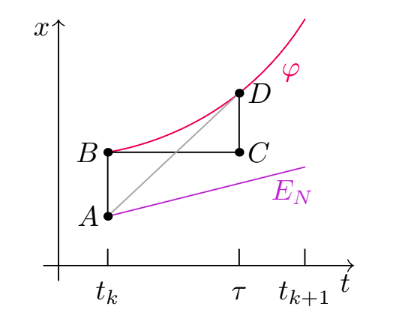
\includegraphics[scale=0.5]{Pics/Screenshot from 2021-01-14 23-23-06.png}}
\end{figure}
\begin{equation*}
    \begin{aligned}
        |(t_k, E_N(t_k)) - (\tau, \varphi(\tau))| &\le |(t_k, E_N(t_k)) - (t_k, \varphi(t_k))| + |(t_k, \varphi(t_k)) - (\tau, \varphi(t_k))| + |(\tau, \varphi(t_k)) - (\tau, \varphi(\tau))| =\\
        &= |E_N(t_k) - \varphi(t_k)| + |t_k - \tau| + |\varphi(t_k) - \varphi(\tau)|
    \end{aligned}
\end{equation*}

Каждое из трех слагаемых можно сделать меньше $\frac{\delta}{3}$ при всех достаточно больших $N$: первое слагаемое --- в силу равномерной сходимости $E_N$ к $\varphi$, второе слагаемое --- в силу того, что оно не превосходит $\frac{h}{N}$, третье слагаемое --- в силу равномерной непрерывности $\varphi$ на $[0, h]$. Отсюда следует (\ref{eulerineq}), что и завершает доказательство теоремы.

\section{Билет №6. Достаточное условие того, что функция удовлетворяет локальному условию Липшица по заданной переменной.}
\textbf{Определение.} Функция $f:\mathbb{R}^m \to \mathbb{R}^n$ удовлетворяет \textbf{условию Липшица} на множестве $D$, если найдется такое число $L$ (\textbf{константа Липшица}), что для любых точек $r_1, r_2 \in D$ выполнено
\begin{equation*}
    |f(r_2) - f(r_1)| \le L|r_2 - r_1|
\end{equation*}

\noindent \textbf{Определение.} Функция $f: \mathbb{R}_{t,r}^{m} \to \mathbb{R}^n$ удовлетворяет \textbf{условию Липшица по $r$ (равномерно по $t$)} на множестве $D$, если найдется такое число $L$, что для любых точек $(t,r_1), (t,r_2) \in D$ справедливо неравенство \begin{equation*}
    |f(t,r_2) - f(t,r_1)| \le L(r_2 - r_1)
\end{equation*}
Обозначается как $f \in Lip_r(D)$.\\

\noindent \textbf{Определение.} Функция $f:\mathbb{R}_{t,r}^{m} \to \mathbb{R}^n$ удовлетворяет \textbf{условию Липшица} по $r$ \textbf{локально} в области $G$, если для любой точки $(t_0, r_0) \in G$ можно указать ее окрестность $U = U(t_0, r_0)$, такую что $f \in Lip_r(U)$. Обозначается как $f \in Lip_{r,loc}(G)$.\\

\noindent \textbf{Лемма.} Пусть $G \subset \mathbb{R}_{t,r}^{n + 1}$ --- область, $f \in C(G \to R^m)$, $f'_r \in M_{m,n}(C(G))$. Тогда $f \in Lip_{r,loc}(G)$.

Кроме того, если $K \subset G$ --- выпуклый компакт,
\begin{equation*}
    M_1 = \max_{(t,r) \in k} |f'_r(t,r)|
\end{equation*}
то для любых $(t,r_1), (t,r_2) \in K$
\begin{equation*}
    |f(t,r_2) - f(t, r_1)| \le nM_1|r_2 - r_1|
\end{equation*}
\textbf{Доказательство.} Рассмотрим произвольные точки $(t,r_1), (t,r_2) \in K$. В силу выпуклости $K$ будет $(t, r + s(r_2 - r_1)) \in K$ при $s \in [0,1]$. Положим
\begin{equation*}
    g(s) = f(t, r_1 + s(r_2 - r_1))
\end{equation*}
Тогда
\begin{equation*}
    \begin{aligned}
        &f(t,r_2) - f(t,r_1) = g(1) - g(0) = \int_0^1 g'(s)ds = \int_0^1 f'_r\cdot r'_sds =\\
        &= \int_0^1 f'_r(t, r_1 + s(r_2 - r_1))\cdot(r_2 - r_1)ds
    \end{aligned}
\end{equation*}
Принимая во внимания леммы о нормах, получаем
\begin{equation*}
    |f(t,r_2) - f(t,r_1)| \le \int_0^1 n|f'_r(t,r_1 + s(r_2 - r_1))||r_2 - r_1|ds \le nM_1|r_2 - r_1|
\end{equation*}
Из этого неравенства можно сделать вывод, что $f \in Lip_r(K)$.

Возьмем произвольную точку $(t_0, r_0) \in G$ и построим замкнутый параллелепипед $B \subset G$ с центром в этой точке. По доказанному $f \in Lip_r(B)$. Так как точка выбрана произвольно, то из этого следует $f \in Lip_{r,loc}(G)$ по определению.

\section{Билет №7. Достаточное условие того, что функция удовлетворяет глобальному условию Липшица по заданной переменной.}
\textbf{Лемма.} Пусть $G \subset \mathbb{R}_{t,r}^{n+1}$ --- область, $f \in C(G \to \mathbb{R}^n)\cap Lip_{r,loc}(G)$, $K \subset G$ --- компакт. Тогда $f \in Lip_r(K)$\\
\noindent \textbf{Доказательство.} Докажем методом от противного. Пусть $f \notin Lip_r(K)$. Тогда для любого $N \in \mathbb{N}$ найдется пара точек $(t_N,r_N), (t_N, \widetilde{r}_N) \in K$, для которых верно неравенство
\begin{equation}
    |f(t_N, r_N) - f(t_N, \widetilde{r}_N)| > N|r_N - \widetilde{r}_N| \label{badlip}
\end{equation}

Поскольку $K$ --- компакт, то из последовательности $\{(t_N, r_N)\}$ можно выбрать подпоследовательность с номерами $\{N_m\}$, сходящуюся к некоторой точке $(t,r) \in K$. Аналогично можно сделать для $\{t_N, \widetilde{r}_N\}$. Далее считаем, что исходная последовательность совпадает с выбранной подпоследовательностью.

Возможны два случая: $r = \widetilde{r}$ и $r \neq \widetilde{r}$.
\begin{enumerate}
    \item $r = \widetilde{r}$. По условию $f \in Lip_{r,loc}(G)$, значит, найдется окрестность $U$ точки $(t,r)$, в которой $f \in Lip_r(U)$, то есть существует постоянная $L$, для которой
    \begin{equation*}
        |f(t', r') - f(t', r'')| \le L|r' - r''|
    \end{equation*}
    при любых $(t',r'), (t',r'') \in U$. Выберем номер $N$ так, чтобы $N > L$ и $(t_N, r_N), (t_N, \widetilde{r}_N) \in U$, и положим $t' = t_N$, $r' = r_N$, $r'' = \widetilde{r}_N$. Тогда из неравенства (\ref{badlip}) следует
    \begin{equation*}
        |f(t',r') - f(t',r'')| > N|r' - r''| \ge L|r' - r''|
    \end{equation*}
    что противоречит условию Липшица.
    \item $r \neq \widetilde{r}$. Выберем непересекающиеся параллелепипеды $R = [a,b] \times X$ и $\widetilde{R} = [a,b] \times \widetilde{X}$, для которых точки $(t,r)$ и $(t,\widetilde{r})$ соответственно являются внутренними. Рассмотрим функцию
    \begin{equation*}
        g(t,x,y) = \frac{|f(t,x) - f(t,y)|}{|x - y|}
    \end{equation*}
    определенную на компакте $[a,b] \times X \times \widetilde{X}$, где она непрерывна, а значит, ограничена некоторым числом $L$. Выбирая номер $N > L$, такой что $(t_N, r_N) \in R$ и $(t_N, \widetilde{r}_N) \in \widetilde{R}$, из (\ref{badlip}) получаем
    \begin{equation*}
        g(t_N, r_N, \widetilde{r}_N) > N > L
    \end{equation*}
    что, естественно, противоречит ограниченности $g$.
\end{enumerate}

\section{Билет №8. Лемма Гронуолла. Теорема Пикара (доказательство единственности решения).}
\textbf{Лемма (Гронуолл).} Пусть $\varphi \in C[a,b]$, $t_0 \in [a,b]$, $\lambda, \mu \ge 0$, при любом $t \in [a,b]$ верно неравенство
\begin{equation*}
    0 \le \varphi(t) \le \lambda + \mu \left|\int_{t_0}^t \varphi(\tau)d\tau\right|
\end{equation*}
Тогда для любого $t \in [a,b]$
\begin{equation*}
    \varphi(t) \le \lambda e^{\mu|t - t_0|}
\end{equation*}
\textbf{Доказательство.} Рассмотрим случай $t \ge t_0$ (при $t < t_0$ доказательство аналогично). Предположим, что $\lambda > 0$ и введем функцию
\begin{equation*}
    v(t) = \lambda + \mu \int_{t_0}^t \varphi(\tau)d\tau
\end{equation*}

Имеем $v(t) > 0$, $v'(t) = \mu\varphi(t) \le \mu v(t)$. Отсюда
\begin{equation*}
    \frac{v'(t)}{v(t)} \le \mu
\end{equation*}
Интегрируя это неравенство по отрезку $[t_0, t]$, получаем
\begin{equation*}
    v(t) \le v(t_0)e^{\mu(t-t_0)}
\end{equation*}
Следовательно,
\begin{equation*}
    \varphi(t) \le v(t) \le v(t_0)e^{\mu(t-t_0)} = \lambda e^{\mu(t-t_0)}
\end{equation*}

Если же $\lambda = 0$, то при любом $\lambda_1 > 0$ верно
\begin{equation*}
    \varphi(t) \le \mu \int_{t_0}^t \varphi(\tau)d\tau \le \lambda_1 + \mu \int_{t_0}^t \varphi(\tau)d\tau
\end{equation*}
По уже доказанному имеем
\begin{equation*}
    \varphi(t) \le \lambda_1 e^{\mu (t - t_0)}
\end{equation*}
Переходя здесь к пределу при $\lambda_1 \to 0$, получаем $\varphi(t) \le 0$. Значит, лемма верна и при $\lambda = 0$.\\

\noindent \textbf{Теорема (Пикар).} Пусть $G \subset \mathbb{R}_{t,r}^{n+1}$ --- область, $f \in C(G \to \mathbb{R}^n) \cap Lip_{r,loc}(G)$, $(t_0, r_0) \in G$. Тогда
\begin{enumerate}
    \item на отрезке Пеано существует решение задачи
    \begin{equation}
        \dot{r} = f(t,r), \quad r(t_0) = r_0 \label{zkpeano1}
    \end{equation}
    \item если $\psi_1$ и $\psi_2$ --- решения (\ref{zkpeano1}) на $(a,b)$, то $\psi_1 \equiv \psi_2$ на $(a,b)$
\end{enumerate}
\textbf{Доказательство (единственность).} Будем считать, что $t_0 = 0$, $r_0 = 0$ (в противном случае перенесем начало координат в точку $(t_0, r_0)$). Пусть $\psi_1$ и $\psi_2$ --- решения (\ref{zkpeano1}). По лемме о равносильном интегральном уравнении имеем
\begin{equation*}
    \psi_1(t) = \int_0^t f(\tau, \psi_1(\tau))d\tau, \quad \psi_2(t) = \int_0^t f(\tau, \psi_2(\tau))d\tau
\end{equation*}
поэтому
\begin{equation*}
    |\psi_1(t) - \psi_2(t)| \le \int_0^t |f(\tau, \psi_1(\tau)) - f(\tau, \psi_2(\tau))|d\tau
\end{equation*}

Рассмотрим произвольный отрезок $[\alpha, \beta] \subset (a,b)$, содержащий ноль. Графики функций $\psi_1$ и $\psi_2$ на $[\alpha, \beta]$ --- компактные множества. Значит по лемме о глобальном условии Липшица найдется постоянная $\widetilde{L}$, такая что
\begin{equation*}
    |f(\tau, \psi_1(\tau)) - f(\tau, \psi_2(\tau))| \le \widetilde{L}|\psi_1(\tau) - \psi_2(\tau)|
\end{equation*}
при всех $\tau \in [\alpha,\beta]$. Следовательно,
\begin{equation*}
    |\psi_1(t) - \psi_2(t)| \le \widetilde{L} \int_0^t |\psi_1(\tau) - \psi_2(\tau)|d\tau
\end{equation*}
По лемме Гронуолла будет $|\psi_1(t) - \psi_2(t)| = 0$ на $[\alpha, \beta]$, то есть $\psi_1 \equiv \psi_2$ на $[\alpha,\beta]$. Так как отрезок $[\alpha, \beta]$ был выбран произвольно, то функции $\psi_1$ и $\psi_2$ совпадают на всем интервале $(a,b)$.

\section{Билет №9. Теорема Пикара (доказательство существования решения).}
\textbf{Теорема (Пикар).} Пусть $G \subset \mathbb{R}_{t,r}^{n+1}$ --- область, $f \in C(G \to \mathbb{R}^n) \cap Lip_{r,loc}(G)$, $(t_0, r_0) \in G$. Тогда
\begin{enumerate}
    \item на отрезке Пеано существует решение задачи
    \begin{equation}
        \dot{r} = f(t,r), \quad r(t_0) = r_0 \label{zkpeano2}
    \end{equation}
    \item если $\psi_1$ и $\psi_2$ --- решения (\ref{zkpeano2}) на $(a,b)$, то $\psi_1 \equiv \psi_2$ на $(a,b)$
\end{enumerate}
\textbf{Доказательство (существование решения).} Будем считать, что $t_0 = 0$, $r_0 = 0$ (в противном случае перенесем начало координат в точку $(t_0, r_0)$). Достаточно установить существование решения на отрезке $[0, h]$ --- правой половине отрезка Пеано. (см. рассуждения в теореме Пеано о существовании решения)

Пусть
\begin{equation*}
    \begin{aligned}
        &\Pi = \left\{(t,r) \in \mathbb{R}^{n + 1}\,|\, |t| \le a,\, |r| \le b\right\} \subset G,\\
        &M = \max_{(t,r) \in \Pi} |f(t,r)|
    \end{aligned}
\end{equation*}
Тогда в качестве $h$ можно взять число $\min \{a, \frac{b}{M}\}$ (см. определение отрезка Пеано).

На отрезке $[0,h]$ зададим последовательность функций
\begin{equation*}
    \begin{aligned}
        &\varphi_0(t) = 0\\
        &\varphi_{k+1} = \int_0^t f(\tau, \varphi_k(\tau))d\tau
    \end{aligned}
\end{equation*}
Дальнейшее изложение доказательства будет состоять из следующих этапов:
\begin{enumerate}
    \item Докажем корректность определения последовательности $\{\varphi_k\}$: чтобы построить функцию $\varphi_{k+1}$ должно быть $(t, \varphi_k(t)) \in G$ при всех $t \in [0,h]$.
    \item Покажем, что последовательность $\{\varphi_k(t)\}$ равномерно на $[0,h]$ сходится к некоторой функции $\varphi$.
    \item Установим, что $\varphi$ --- решение интегрального уравнения, равносильного задаче (\ref{zkpeano2})
\end{enumerate}

\begin{enumerate}
    \item При $k = 0$ очевидно, $(t, \varphi_k(t)) \in G$. Допустим справедливость этого утверждения при некотором $k$. Тогда функция $\varphi_{k+1}$ определена на $[0,h]$ и
    \begin{equation*}
        |\varphi_{k+1}(t)| \le \int_0^t |f(\tau, \varphi_k(\tau))|d\tau \le Mt \le Mh \le M\frac{b}{M} = b
    \end{equation*}
    что влечет включение $(t, \varphi_{k+1}(t)) \in \Pi \subset G$ при всех $t \in [0,h]$
    \item Воспользуемся критерием Коши. А именно, установим, что для любого $\varepsilon > 0$ найдется $N \in \mathbb{N}$, такое что при всех $m \ge N$, всех $k \in \mathbb{N}$ и всех $t \in [0,h]$
    \begin{equation*}
        |\varphi_{m+k}(t) - \varphi_m(t)| \le \varepsilon
    \end{equation*}
    По лемме о глобальном условии Липшица будет $f \in Lip_r(\Pi)$ с некоторой константой Липшица $L$. Индукцией по $m$ докажем неравенство
    \begin{equation}
        |\varphi_{m+k}(t) - \varphi_m(t)| \le \frac{ML^mt^{m+1}}{(m+1)!} \label{ind}
    \end{equation}
    При $m = 0$ утверждение верно, так как
    \begin{equation*}
        |\varphi_k(t) - \varphi_0(t)| \le \int_0^t |f(\tau, \varphi_{k-1}(\tau))|d\tau \le Mt
    \end{equation*}
    Допуская его справедливость при некотором $m$, имеем
    \begin{equation*}
        \begin{aligned}
            &|\varphi_{m + 1 + k}(t) - \varphi_{m+1}(t)| \le \int_0^t |f(\tau, \varphi_{m+k}(\tau)) - f(\tau, \varphi_m(\tau))|d\tau \le \\
            &\le \int_0^t L|\varphi_{m+k}(\tau) - \varphi_m(\tau)|d\tau \le \int_0^t L\frac{ML^m\tau^{m+1}}{(m+1)!}d\tau = \frac{ML^{m+1}t^{m+2}}{(m+2)!}
        \end{aligned}
    \end{equation*}
    что и требовалось. Из (\ref{ind}) вытекает, что при любом $t \in [0,h]$
    \begin{equation}
        |\varphi_{m+k}(t) - \varphi_m(t)| \le \frac{ML^mh^{m+1}}{(m+1)!} \label{indh}
    \end{equation}
    Выражение в правой части не зависит от $t$ и $k$ и стремится к нулю при $m \to \infty$, поскольку оно является общим членом ряда Тейлора для экспоненты. Значит, последовательность $\{\varphi_m\}$ удовлетворяет критерию Коши. Обозначим через $\varphi$ ее предел на $[0,h]$.
    \item Переходя к пределу при $m \to \infty$ в равенстве
    \begin{equation*}
        \varphi_{m+1}(t) = \int_0^t f(\tau, \varphi_m(\tau))d\tau
    \end{equation*}
    получаем
    \begin{equation}
        \varphi(t) = \lim_{m \to \infty} \int_0^t f(\tau, \varphi_m(\tau))d\tau \label{lim}
    \end{equation}
    
    В первом пункте было установлено, что $(t, \varphi_m(t)) \in \Pi$ при всех $t \in [0,h]$. Тогда при $m \to \infty$ будет $(t, \varphi(t)) \in \Pi$ при всех таких $t$. Следовательно,
    \begin{equation*}
        |f(\tau, \varphi_m(\tau)) - f(\tau, \varphi(\tau))| \le L|\varphi_m(\tau) - \varphi(\tau)|
    \end{equation*}
    Учитывая равномерную сходимость $\varphi_m$, из данного неравенства следует, что $f(t, \varphi_m(t)) \to f(t, \varphi(t))$ при $m \to \infty$ равномерно на $[0,h]$. Это позволяет внести знак предела под интеграл в (\ref{lim}). После этого по лемме о равносильном интегральном уравнении заключаем, что $\varphi$ --- решение задачи (\ref{zkpeano2}) на $[0,h]$.
\end{enumerate}

\section{Билет №10. Теорема существования и единственности решения ЗК для уравнения n-го
порядка. Следствие с более простыми условиями.}
\textbf{Теорема (Пикар).} Пусть $G \subset \mathbb{R}_{t,r}^{n+1}$ --- область, $f \in C(G \to \mathbb{R}^n) \cap Lip_{r,loc}(G)$, $(t_0, r_0) \in G$. Тогда
\begin{enumerate}
    \item на отрезке Пеано существует решение задачи
    \begin{equation}
        \dot{r} = f(t,r), \quad r(t_0) = r_0 \label{zkpeano3}
    \end{equation}
    \item если $\psi_1$ и $\psi_2$ --- решения (\ref{zkpeano3}) на $(a,b)$, то $\psi_1 \equiv \psi_2$ на $(a,b)$
\end{enumerate}

\noindent \textbf{Следствие (Теорема Пикара с простыми условиями).} Пусть $G \subset \mathbb{R}_{t,r}^{n+1}$ --- область, $f \in C(G \to \mathbb{R}^n)$, $f'_r \in M_n(C(G))$, $(t_0, r_0) \in G$. Тогда
\begin{enumerate}
    \item на отрезке Пеано $[t_0 - h, t_0 + h]$ существует решение $\varphi$ ЗК
    \item если $\psi_1$ и $\psi_2$ --- решения этой задачи на $(a,b)$, то $\psi_1 \equiv \psi_2$ на $(a,b)$
    \item пусть $\Pi$ --- параллелепипед, по которому строится отрезок Пеано,
    \begin{equation*}
        M = \max_{(t,r) \in \Pi} |f(t,r)|, \quad M_1 = \max_{(t,r) \in \Pi} |f'_r(t,r)|
    \end{equation*}
    $\varphi_m$ --- $m$-е приближение Пикара, тогда для любого $t \in [t_0 - h, t_0 + h]$
    \begin{equation*}
        |\varphi(t) - \varphi_m(t)| \le \frac{M(nM_1)^mh^{m+1}}{(m+1)!}
    \end{equation*}
\end{enumerate}
\textbf{Доказательство.} Пункты (1) и (2) следуют из леммы о локальном условии Липшица и теоремы Пикара. Для доказательства пункта (3) сделаем предельный переход в неравенстве (\ref{indh}) при $k \to \infty$. Тогда
\begin{equation*}
    |\varphi(t) - \varphi_m(t)| \le \frac{ML^mh^{m+1}}{(m+1)!}
\end{equation*}
По лемме о локальном условии Липшица в качестве $L$ можно взять $nM_1$.

\section{Билет №11. Критерий продолжимости.}
\textbf{Определение.} Решение $\varphi$ уравнения $\dot{r} = f(t,r)$ на промежутке $\langle a,b \rangle$ называется \textbf{продолжимым}, если существует решение $\psi$ того же уравнения на промежутке $\langle A, B \rangle$, причем $\langle a,b \rangle \subset \langle A,B \rangle$ и $\varphi \equiv \psi$ на $\langle a,b \rangle$. Решение $\psi$ называют \textbf{продолжением} решения $\varphi$.\\

\noindent \textbf{Определение.} Если для решения $\varphi$ уравнения $\dot{r} = f(t,r)$ не существует продолжения, то будем называть функцию $\varphi$ \textbf{максимальным решением}.\\

\noindent \textbf{Теорема (Критерий продолжимости).} Пусть $G \subset \mathbb{R}_{t,r}^{n+1}$ --- область, $f \in C(G \to \mathbb{R}^{n})$. Тогда решение $\varphi$ уравнения $\dot{r} = f(t,r)$ на промежутке $[a,b)$ продолжимо вправо, если и только если существует предел $\varphi(b - 0) = \widetilde{r}$ и $(b, \widetilde{r}) \in G$.\\

\noindent \textbf{Доказательство.} Предположим, что $\psi$ --- продолжение на $[a,c\rangle$ решения $\varphi$, $b \in [a,c\rangle$. Тогда в силу непрерывности $\psi$
\begin{equation*}
    \varphi(b-0) = \psi(b-0) = \psi(b)
\end{equation*}
Поскольку $b \in [a,c\rangle$, то из определения решения следует $(b, \psi(b)) \in G$.

Докажем обратное утверждение. Доопределим функцию $\varphi$ по непрерывности на промежуток $[a,b]$. При $t,t_1 \in [a,b)$
\begin{equation*}
    \varphi(t) - \varphi(t_1) = \int_{t_1}^t \varphi'(\tau)d\tau = \int_{t_1}^t f(\tau, \varphi(\tau))d\tau
\end{equation*}
Переходя к пределу при $t_1 \to t_0$, получаем
\begin{equation*}
    \varphi(t) = \widetilde{r} + \int_{t_0}^t f(\tau, \varphi(\tau))d\tau
\end{equation*}
Тогда по лемме о равносильном интегральном уравнении функция $\varphi$ --- решение задачи
\begin{equation}
    \dot{r} = f(t,r), \quad r(b) = \widetilde{r} \label{zktilde}
\end{equation}

По теореме Пеано существует ее решение $\chi$ на некотором отрезке $[b-h, b+h]$. Положим
\begin{equation*}
    \psi(t) = \begin{cases}
    \varphi(t), t \in [a,b)\\
    \chi(t), t \in [b, b + h]
    \end{cases}
\end{equation*}

По лемме о гладкой стыковке решений функция $\psi$ --- решение задачи (\ref{zktilde}) на $[a,b+h]$, следовательно, $\psi$ --- продолжение решения $\varphi$ вправо за точку $b$.

\section{Билет №12. Теорема существования и единственности максимального решения.}
\textbf{Теорема.} Пусть $G \subset \mathbb{R}_{t,r}^{n+1}$ --- область, $f \in C(G \to \mathbb{R}^{n}) \cap Lip_{r,loc}(G)$, $(t_0, r_0) \in G$. Тогда максимальное решение ЗК $\dot{r} = f(t,r),\, r(t_0) = r_0$ существует и единственно.\\

\noindent \textbf{Доказательство.} Рассмотрим множество $S$ всевозможных решений ЗК, определенных на интервалах. По теореме Пеано это множество не пусто. Обозначим через $(a_{\varphi}, b_{\varphi})$ область определения решения $\varphi \in S$. Положим
\begin{equation*}
    (A,B) = \bigcup_{\varphi \in S}(a_{\varphi}, b_{\varphi})
\end{equation*}

Определим на $(A,B)$ функцию $\psi$ следующим образом. Если $t \in (A,B)$, то найдется функция $\varphi \in S$, такая что $t \in (a_{\varphi}, b_{\varphi})$. Тогда положим $\psi(t) = \varphi(t)$. Определение корректно, поскольку значение в точке $t$ любой другой функции из $S$, определенной в $t$, совпадает с $\varphi(t)$ по теореме Пикара.

Отсюда следует, что $\psi \equiv \varphi$ на $(a_{\varphi}, b_{\varphi})$. А раз $\varphi$ --- решение, то $\psi$ непрерывно дифференцируема в $t$ и $\dot{\psi}(t) = \dot{\varphi}(t) = f(t,\varphi(t)) = f(t,\psi(t))$. В силу произвольности выбора точки $t$ получаем
\begin{itemize}
    \item $\psi \in C^1(A,B)$
    \item $\dot{\psi} = f(t,\psi(t))$ при всех $t \in (A,B)$
\end{itemize}
Кроме того, $\psi(t_0) = \varphi(t_0) = r_0$. Тогда $\psi$ --- решение исходной ЗК по определению.

Поскольку интервал $(A,B)$ включает в себя все возможные интервалы, на которых могут быть заданы решения, то $\psi$ является максимальным решением.

Другого максимального решения быть не может. Докажем от противного. Пусть имеется еще одно максимальное решение $\widetilde{\psi}:\, (\widetilde{A}, \widetilde{B}) \to \mathbb{R}^n$. Тогда $(\widetilde{A}, \widetilde{B}) \subset (A,B)$ и $\widetilde{\psi} \equiv \psi$ на $(\widetilde{A}, \widetilde{B})$. Если, например, $\widetilde{B} < B$, то $\psi$ --- продолжение $\widetilde{\psi}$ вправо, что противоречит непродолжимости решения $\widetilde{\psi}$.

\section{Билет №13. Теорема о выходе интегральной кривой за пределы любого компакта.}
\textbf{Теорема.} Пусть $n \in \mathbb{N}$, $G \subset \mathbb{R}_{t,r}^{n+1}$ --- область, $f \in C(G \to \mathbb{R}^n)\cap Lip_{r,loc}(G)$, $\varphi$ --- максимальное решение на $(a,b)$ уравнения $\dot{r} = f(t,r)$, $K \subset G$ --- компакт. Тогда найдется $\Delta > 0$, такое что $(t, \varphi(t)) \notin K$ при всех $t \in (a, a + \Delta) \cup (b - \Delta, b)$.\\

\noindent \textbf{Доказательство.} Заметим, что расстояние $\rho = \rho(K, \partial G)$ от компакта $K$ до границы $\partial G$ области $G$ положительно (иначе можно было бы построить последовательность точек из $K$, сходящейся к точке на границе, но $\partial G \cap K = \varnothing$). Если $\rho < +\infty$, положим $c = \frac{\rho}{2}$, иначе пусть $c = 1$.

Вокруг каждой точки $(t', r') \in K$ построим содержащийся внутри $G$ параллелепипед
\begin{equation*}
    \Pi(t',r') = \left\{(t,r) \in \mathbb{R}^{n+1}\, | \, |t-t'| \le c,\, |r - r'| \le c \right\}
\end{equation*}
и рассмотрим множество
\begin{equation*}
    K_c = \bigcup_{(t',r') \in K} \Pi(t',r')
\end{equation*}

Поскольку $K$ --- компакт, то норма каждого элемента из $K$ ограничена некоторым числом $d$. Если $(t,r)$ --- произвольная точка из $K_c$, то для некоторой точки $(t',r') \in K$ будет $(t,r) \in \Pi(t',r')$, поэтому
\begin{equation*}
    |(t,r)| \le |(t,r) - (t',r')| + |(t',r')| \le c + d
\end{equation*}
Значит, множество $K_c$ ограничено.

Докажем его замкнутость. Рассмотрим последовательность $\{(t_{m_k}, r_{m_k})\}$ точек из $K_c$, сходящуюся к $(t,r) \in \mathbb{R}^{n+1}$. Для каждой такой точки найдется параллелепипед $\Pi(t'_{m_k},r'_{m_k})$, которому она принадлежит. Раз $K$ --- компакт, то существует подпоследовательность $\{(t'_{m_k}, r'_{m_k})\}$, сходящаяся к некоторой точке $(t',r') \in K$. Переходя к пределу в неравенствах
\begin{equation*}
    |t_{m_k} - t'_{m_k}| \le c, \quad |r_{m_k} - r'_{m_k}| \le c
\end{equation*}
находим $|t - t'| \le c$ и $|r - r'| \le c$. Следовательно $(t,r) \in K_c$.

Таким образом, $K_c$ --- компакт, и функция $f$ достигает на нем максимального значения
\begin{equation*}
    M = \max_{(t,r) \in K_c} |f(t,r)|
\end{equation*}

Теперь предположим, что утверждение теоремы неверно. Пусть $\Delta = \frac{h}{2}$, где $h = \min \{c, \frac{c}{M}\}$. Тогда при некотором $t_0 \in (b - \frac{h}{2}, b)$ будет $(t_0, \varphi(t_0)) \in K$.

Рассмотрим ЗК $\dot{r} = f(t,r),\, r(t_0) = \varphi(t_0)$. По теореме Пеано она имеет решение $\psi$ на отрезке $[t_0 - h, t_0 + h]$. Пусть
\begin{equation*}
    \widetilde{\varphi}(t) = \begin{cases}
    \varphi(t), \quad \text{если } t \in (a, t_0)\\
    \psi(t), \quad \text{если } t \in [t_0, t_0 + h]
    \end{cases}
\end{equation*}

По лемме о гладкой стыковке решений $\widetilde{\varphi}$ --- решение уравнения $\dot{r} = f(t,r)$ на $(a, t_0 + h)$. Функция $\widetilde{\varphi} \equiv \varphi$ на $(a,b) \cap (a, t_0 + h)$ по теореме Пикара. Но
\begin{equation*}
    t_0 + h > b - \frac{h}{2} + h = b + \frac{h}{2} > b
\end{equation*}
то есть $\widetilde{\varphi}$ --- продолжение $\varphi$ вправо за точку $b$. Так как $\varphi$ по условию является максимальным решением, приходим к противоречию.

\section{Билет №14. Признак продолжимости решения системы, сравнимой с линейной. Теорема о существовании и единственности максимального решения ЛС.}
\textbf{Теорема (О системе, сравнимой с линейной).} Пусть $G = (a,b) \times \mathbb{R}_r^n$, $f \in C(G \to \mathbb{R}^n) \cap Lip_{r,loc}(G)$, функции $u,v \in C(a,b)$ таковы, что для любых $(t,r) \in G$
\begin{equation*}
    |f(t,r)| \le u(t)|r| + v(t)
\end{equation*}
Тогда каждое максимальное решение уравнения $\dot{r} = f(t,r)$ определено на $(a,b)$.\\

\noindent \textbf{Доказательство.} По теореме о существовании и единственности максимального решения любая задача Коши с начальными данными $(t_0, r_0) \in G$ имеет единственное максимальное решение $\varphi$, заданное на некотором интервале $(\alpha, \beta)$. Докажем, что границы интервала $(\alpha, \beta)$ совпадают с границами интервала $(a,b)$. Пойдем от противного. Пусть, например, $\beta < b$. Принимая во внимание лемму о равносильном интегральном уравнении, при $t \in [t_0, \beta)$ находим
\begin{equation*}
    \begin{aligned}
        &|\varphi(t)| = \left|r_0 + \int_{t_0}^t f(\tau, \varphi(\tau))d\tau \right| \le |r_0| + \int_{t_0}^t |f(\tau, \varphi(\tau))|d\tau \le\\
        &\le |r_0| + \int_{t_0}^t |u(\tau)||\varphi(\tau)|d\tau + \int_{t_0}^t |v(\tau)|d\tau
    \end{aligned}
\end{equation*}

Из непрерывности функций $u$ и $v$ вытекает их ограниченность на отрезке $[t_0, \beta]$. Следовательно, найдутся такие числа $\lambda, \mu \ge 0$, что при $t \in [t_0, \beta)$
\begin{equation*}
    |\varphi(t)| \le \lambda + \mu \int_{t_0}^t |\varphi(s)|ds
\end{equation*}
Тогда по лемме Гронуолла
\begin{equation*}
    |\varphi(t)| \le \lambda e^{\mu (t - t_0)} \le L
\end{equation*}
где $L = \lambda e^{\mu (\beta - t_0)}$. Отсюда следует, что график решения $\varphi$ не покидает компакт
\begin{equation*}
    K = \left\{(t,r) \in G\, |\, t \in [t_0, \beta],\, |r| \le L \right\} \subset G
\end{equation*}
при $t \in [t_0, \beta)$, что противоречит теореме о выходе интегральной кривой за пределы компакта.\\

\noindent \textbf{Определение.} \textbf{Линейной системой дифференциальных уравнений} называют систему вида
\begin{equation}
    \dot{r} = P(t)r + q(t) \label{lnsu}
\end{equation}
где $P \in M_n(C(a,b))$, $q \in C((a,b) \to \mathbb{R}^n)$.\\

\noindent \textbf{Теорема (существование и единственность максимального решения ЛС).} Пусть $P \in M_n(C(a,b))$, $q \in C((a,b) \to \mathbb{R}^n)$, $t_0 \in (a,b)$, $r_0 \in \mathbb{R}^n$. Тогда максимальное решение задачи Коши
\begin{equation}
    \begin{cases}
    \dot{r} = P(t)r + q(t)\\
    r(t_0) = r_0
    \end{cases} \label{zkls}
\end{equation}
существует, единственно и определено на интервале $(a,b)$.\\

\noindent \textbf{Доказательство.} Заметим, что правая часть системы $f(t,r) = P(t)r + q(t)$ и ее производная $f'_r = P(t)$ непрерывны в области $(a,b) \times \mathbb{R}^n$. Тогда существует единственное максимальное решение задачи (\ref{zkls}).

Имеем
\begin{equation*}
    |f(t,r)| \le |P(t)r| + |q(t)| \le n|P(t)||r| + |q(t)|
\end{equation*}
Так как функции $u(t) = n|P(t)|$ и $v(t) = |q(t)|$ непрерывны на $(a,b)$, то по признаку продолжимости системы, сравнимой с линейной, решение задачи (\ref{zkls}) продолжимо на интервал $(a,b)$.

\section{Билет №15. Формула Остроградского–Лиувилля для решений ЛОС.}
\textbf{Определение.} Если $q \equiv 0$ на $(a,b)$, то система (\ref{lnsu}), то есть
\begin{equation}
    \dot{r} = P(t)r \label{losu}
\end{equation}
называется \textbf{однородной}, в противном случае \textbf{неоднородной}.\\

\noindent \textbf{Определение.} \textbf{Определителем Вронского (вронскианом)} вектор-функций $\{r_k\}_{k=1}^n$, где $r_k=(x_{k1}, x_{k2}, \ldots, x_{kn})^T$, называют определитель
\begin{equation*}
    W(t) = det(r_1(t),r_2(t),\ldots, r_n(t)) = \begin{vmatrix}
    x_{11}(t) & x_{21}(t) & \ldots & x_{n1}(t)\\
    x_{12}(t) & x_{22}(t) & \ldots & x_{n2}(t)\\
    \ldots\\
    x_{1n}(t) & x_{2n}(t) & \ldots & x_{nn}(t)
    \end{vmatrix}
\end{equation*}
\\
\noindent \textbf{Теорема (формула Остроградского-Лиувилля для решений ЛОС).} Пусть $t, t_0 \in (a,b)$, $P \in M_n(C(a,b))$, $r_1, r_2, \ldots, r_n$ --- решения системы (\ref{losu}). Тогда их вронскиан
\begin{equation*}
    W(t) = W(t_0)\exp \int_{t_0}^t trP(\tau)d\tau
\end{equation*}
\textbf{Доказательство.} Пусть $X$ --- матрица со столбцами $r_1, r_2, \ldots, r_n$, а $R_k$ --- ее $k$-ая строка. Используя формулу полного разложения определителя, нетрудно убедиться, что
\begin{equation*}
    \dot{W} = det\begin{pmatrix}
    \dot{R}_1\\
    R_2\\
    \ldots\\
    R_n
    \end{pmatrix} + det\begin{pmatrix}
    R_1\\
    \dot{R}_2\\
    \ldots\\
    R_n
    \end{pmatrix} + \ldots + det\begin{pmatrix}
    R_1\\
    R_2\\
    \ldots\\
    \dot{R}_n
    \end{pmatrix}
\end{equation*}

Так как
\begin{equation*}
    \dot{X} = (\dot{r}_1, \dot{r}_2, \ldots, \dot{r}_n) = (Pr_1, Pr_2, \ldots, Pr_n) = PX
\end{equation*}
то $k$-ая строка матрицы $\dot{X}$ совпадает с $k$-ой строкой матрицы $PX$, то есть
\begin{equation*}
    \dot{R}_k = \sum_{k=1}^n p_{kj}R_j
\end{equation*}
где $p_{kj}$ --- элемент матрицы $P$ в $k$-ой строке и $j$-ом столбце.

Подставляя выражение для $\dot{R}_k$ в формулу для $\dot{W}$ и используя свойства определителя, находим
\begin{equation*}
    \dot{W} = p_{11}det\begin{pmatrix}
    R_1\\
    R_2\\
    \ldots\\
    R_n
    \end{pmatrix} + p_{22}det\begin{pmatrix}
    R_1\\
    R_2\\
    \ldots\\
    R_n
    \end{pmatrix} + \ldots + p_{nn}det\begin{pmatrix}
    R_1\\
    R_2\\
    \ldots\\
    R_n
    \end{pmatrix} = W\,trP
\end{equation*}
Интегрируя полученное уравнение, приходим к требуемой формуле.

\section{Билет №16. Общее решение ЛОС. Лемма о множестве фундаментальных матриц. Лемма об овеществлении.}
\textbf{Теорема (Общее решение ЛОС).} Пусть $P \in M_n(C(a,b))$. Тогда множество решений системы $\dot{r} = P(t)r$ образуют $n$-мерное линейное пространство.\\

\noindent \textbf{Доказательство.} Пусть $t_0 \in (a,b)$, $\{a_k\}_{k=1}^n$ --- базис в $\mathbb{R}^n$. Тогда для любого $k \in [1 : n]$ существует $r_k$ --- решение задачи Коши $\dot{r} = P(t)r,\, r(t_0) = a_k$. Вронскиан этих решений $W(t_0) = det(a_1, a_2, \ldots, a_n) \neq 0$. Тогда функции $\{r_k\}_{k=1}^n$ линейно независимы.

Рассмотрим произвольное решение $r$ системы $\dot{r} = P(t)r$. Пусть $\{c_k\}_{k=1}^n$ --- координаты вектора $r(t_0)$ в базисе $\{a_k\}_{k=1}^n$. Положим
\begin{equation*}
    \varphi = c_1r_1 + c_2r_2 + \ldots + c_nr_n
\end{equation*}
Ясно, что $\varphi$ --- решение системы $\dot{r} = P(t)r$, при этом $\varphi(t_0) = r_0$. Тогда $r \equiv \varphi$ в силу теоремы о единственности максимального решения ЛС.

Таким образом, функции $\{r_k\}_{k=1}^n$ линейно независимы, и любое решение есть их линейная комбинация. Значит, $\{r_k\}_{k=1}^n$ --- базис в пространстве решений.\\

\noindent \textbf{Определение.} \textbf{Фундаментальной системой решений} системы уравнений $\dot{r} = P(t)r$ называется совокупность ее $n$ линейно независимых решений.\\

\noindent \textbf{Определение.} \textbf{Фундаментальная матрица системы} $\dot{r} = P(t)r$ --- матрица, столбцы которой образуют фундаментальную систему решений.\\

\noindent \textbf{Лемма (о множестве фундаментальных матриц).} Пусть $\Phi$ --- фундаментальная матрица системы $\dot{r} = P(t)r$. Тогда $\left\{\Phi A \, | \, A \in M_n(\mathbb{R}), \, detA \neq 0 \right\}$ --- множество всех фундаментальных матриц этой системы.\\

\noindent \textbf{Доказательство.} Пусть $\Psi$ --- фундаментальная матрица системы $\dot{r} = P(t)r$. Тогда каждый ее столбец, будучи решением этой системы, является линейной комбинацией столбцов матрицы $\Phi$. Записывая коэффициенты разложения в столбцы матрицы $A$, имеем $\Psi = \Phi A$. А так как $det \Psi \neq 0$ и $\det \Phi \neq 0$, то и $det A \neq 0$.

Обратно, пусть $A \in M_n(\mathbb{R})$ --- произвольная невырожденная матрица. Тогда матрица $\Phi A$ состоит из решений, а ее определитель не обращается в ноль. Следовательно, эти решения линейно независимы, поэтому $\Phi A$ --- фундаментальная матрица.\\

\noindent \textbf{Лемма (Об овеществлении).} Пусть $n \in \mathbb{N}$, $\Phi = (r_1,r_2,r_3,\ldots,r_n)$ --- фундаментальная матрица системы $\dot{r} = P(t)r$, при этом $r_1 = \overline{r}_2$. Тогда
\begin{equation*}
    \Psi = (Re\,r_1, Im\,r_1, r_3, \ldots, r_n)
\end{equation*}
--- фундаментальная матрица той же системы.\\

\noindent \textbf{Доказательство.} Так как
\begin{equation*}
    \begin{aligned}
        &Re\, r_1 = \frac{1}{2}(r_1 + \overline{r}_1) = \frac{1}{2}r_1 + \frac{1}{2}r_2\\
        &Im\,r_1 = \frac{1}{2i}(r_1 - \overline{r}_1) = \frac{1}{2i}r_1 - \frac{1}{2i}r_2
    \end{aligned}
\end{equation*}
то
\begin{equation*}
    \Psi = \Phi \begin{pmatrix}
    \begin{matrix}
    \frac{1}{2} & \frac{1}{2i}\\
    \frac{1}{2} & -\frac{1}{2i}
    \end{matrix} & 0\\
    0 & E_{n-2}
    \end{pmatrix}
\end{equation*}
где $E_{n-2}$ --- единичная матрица порядка $n - 2$. По лемме о множестве фундаментальных матриц матрица $\Psi$ является фундаментальной.

\section{Билет №17. Теорема о фундаментальной системе решений ЛОС с постоянными коэффициентами (случай жорданова базиса общего вида). Определение и свойства матричной экспоненты (без доказательств). Решение задачи Коши при помощи матричной экспоненты.}
\textbf{Определение.} \textbf{Линейной системой дифференциальных уравнений с постоянными коэффициентами} называют линейную систему вида
\begin{equation}
    \dot{r} = Ar = q(t) \label{linpost}
\end{equation}
где $A \in M_n(\mathbb{C})$, $q \in C((a,b) \to \mathbb{C}^n)$.\\

\noindent \textbf{Лемма.} Пусть $n, k \in \mathbb{N}$, $A \in M_n(\mathbb{C})$, $h_1, h_2, \ldots, h_k$ --- жорданова цепочка, соответствующая $\lambda \in spec\, A$. Тогда функции
\begin{equation*}
    \begin{aligned}
        &\varphi_1(t) = e^{\lambda t}h_1\\
        &\varphi_2(t) = e^{\lambda t}\left(\frac{t}{1!}h_1 + h_2\right)\\
        &\ldots\\
        &\varphi_k(t) = e^{\lambda t}\left(\frac{t^{k-1}}{(k-1)!}h_1 + \ldots + \frac{t}{1!}h_{k-1} + h_k\right)
    \end{aligned}
\end{equation*}
являются решениями системы $\dot{r} = Ar$.\\

\noindent \textbf{Доказательство.} Принимая во внимание определение жордановой цепочки, при $j \in [1 : k]$ имеем
\begin{equation*}
    \begin{aligned}
        &A\varphi_j = e^{\lambda t}\sum_{m=1}^j \frac{t^{j-m}}{(j-m)!}Ah_m = e^{\lambda t} \left(\frac{t^{j-1}}{(j-1)!}\lambda h_1 + \sum_{m=2}^j \frac{t^{j-m}}{(j-m)!}(\lambda h_m + h_{m - 1}) \right) = \\
        &= e^{\lambda t}\left(\lambda \sum_{m=1}^j \frac{t^{j - m}}{(j - m)!}h_m + \sum_{m = 2}^j \frac{t^{j-m}}{(j - m)!}h_{m-1} \right)
    \end{aligned}
\end{equation*}

Это же выражение получается при дифференцировании вектор-функции $\varphi_j$. Значит, $\dot{\varphi}_j = A\varphi_j$, что и требовалось доказать.\\

\noindent \textbf{Теорема (Случай жорданова базиса общего вида).} Пусть $A \in M_n(\mathbb{C})$, базис пространства $\mathbb{C}^n$ состоит из жордановых цепочек
\begin{equation*}
    \begin{aligned}
        &\lambda_1 \sim h_1, h_2, \ldots, h_k\\
        &\ldots\\
        &\lambda_d \sim u_1, u_2, \ldots, u_m
    \end{aligned}
\end{equation*}
соответствующих $\lambda_1, \ldots, \lambda_d \in spec\, A$. Тогда вектор-функции
\begin{equation*}
    \begin{aligned}
        &\varphi_1(t) = e^{\lambda_1 t}h_1, \quad \ldots, \quad \varphi_k(t) = e^{\lambda_1 t}\left(\frac{t^{k-1}}{(k-1)!}h_1 + \ldots + \frac{t}{1!}h_{k-1} + h_k \right)\\
        &\ldots\\
        &\psi_1(t) = e^{\lambda_d t}u_1, \quad \ldots, \quad \psi_m(t) = e^{\lambda_d t}\left(\frac{t^{m-1}}{(m-1)!}u_1 + \ldots + \frac{t}{1!}u_{m-1} + u_m \right)
    \end{aligned}
\end{equation*}
образуют фундаментальную систему решений системы $\dot{r} = Ar$.\\

\noindent \textbf{Доказательство.} По вышедоказанной лемме каждая из вектор-функций
\begin{equation*}
    \varphi_1, \ldots, \varphi_k, \ldots, \psi_1, \ldots, \psi_m
\end{equation*}
является решением. Их вронскиан
\begin{equation*}
    W(0) = det(h_1, \ldots, h_k, \ldots, u_1, \ldots, u_m) \neq 0
\end{equation*}
Тогда вектор-функции $\{\varphi_1, \ldots, \varphi_k, \ldots, \psi_1, \ldots, \psi_m\}$ линейно независимы, а значит, образуют фундаментальную систему решений.\\

\noindent \textbf{Определение.} \textbf{Матричной экспонентой} называется сумма ряда
\begin{equation*}
    e^{A} = \sum_{k = 0}^{\infty} \frac{A^k}{k!}
\end{equation*}
\\
\noindent \textbf{Свойства матричной экспоненты.} Пусть $A$, $B$, $J$, $T \in M_n(\mathbb{C})$, $det\, T \neq 0$, $t \in \mathbb{R}$. Тогда
\begin{enumerate}
    \item ряд, определяющий $e^A$, сходится
    \item если $AB = BA$, то $e^{A+B} = e^{A}e^{B}$
    \item $\frac{d}{dt}e^{At} = Ae^{At}$
    \item если $A = TJT^{-1}$, то $e^A = Te^JT^{-1}$
    \item если $A = diag(A_1, A_2, \ldots, A_d)$, то $e^A = diag(e^{A_1}, e^{A_2}, \ldots, e^{A_d})$
    \item если $J_s(\lambda)$ --- жорданова клетка размера $s$:
    \begin{equation*}
        J_s(\lambda) = \begin{pmatrix}
            \lambda & 1 & 0 & \ldots & 0\\
            0 & \lambda & 1 & \ldots & 0\\
            0 & 0 & \lambda & \ldots & 0\\
            \ldots\\
            0 & 0 & 0 & \ldots & \lambda
        \end{pmatrix}
    \end{equation*}
    то
    \begin{equation*}
        e^{J_s(\lambda)t} = \begin{pmatrix}
        1 & t & \frac{t^2}{2!} & \ldots & \frac{t^{s-1}}{(s-1)!}\\
        0 & 1 & t & \ldots & \frac{t^{s-2}}{(s-2)!}\\
        0 & 0 & 1 & \ldots & \frac{t^{s-3}}{(s-3)!}\\
        \ldots\\
        0 & 0 & 0 & \ldots & 1
        \end{pmatrix}
    \end{equation*}
\end{enumerate}
\\
\noindent \textbf{Теорема.} Пусть $A \in M_n(\mathbb{C})$. Тогда матрица $e^{At}$ является фундаментальной матрицей системы $\dot{r} = Ar$.\\

\noindent \textbf{Доказательство.} По свойствам матричной экспоненты будет $\frac{d}{dt}e^{At} = Ae^{At}$. Следовательно, каждый столбец матрицы $e^{At}$ --- решение системы $\dot{r} = Ar$. Соответствующий вронскиан
\begin{equation*}
    W(0) = det\, e^{A\cdot 0} = det\, E_n = 1
\end{equation*}
где $E_n$ --- единичная матрица порядка $n$. Отсюда следует, что $e^{At}$ --- фундаментальная матрица.\\

\noindent \textbf{Следствие.} Пусть $A \in M_n(\mathbb{C})$, $t_0 \in \mathbb{R}$, $r_0 \in \mathbb{C}^n$. Тогда решением задачи
\begin{equation*}
    \dot{r} = Ar, \quad r(t_0) = r_0
\end{equation*}
является вектор-функция $\varphi(t) = e^{A(t - t_0)}r_0$

\section{Билет №18. Общее решение ЛНС и метод вариации постоянных.}
\textbf{Теорема (Общее решение ЛНС).} Пусть $P \in M_n(C(a,b))$, $q \in C((a,b) \to \mathbb{R}^n)$, $\varphi$ --- решение системы
\begin{equation}
    \dot{r} = P(t)r + q(t) \label{lnusyst2}
\end{equation}
$\Phi$ --- фундаментальная матрица системы
\begin{equation*}
    \dot{r} = P(t)r
\end{equation*}
Тогда общее решение неоднородной системы (\ref{lnusyst2}) имеет вид
\begin{equation*}
    r = \Phi C + \varphi, \quad C \in \mathbb{R}^n
\end{equation*}
\textbf{Доказательство.} Пусть $r$ --- произвольное решение (\ref{lnusyst2}). Тогда
\begin{equation*}
    \dot{r} = Pr + q
\end{equation*}
Функция $\varphi$ удовлетворяет такому же соотношению:
\begin{equation*}
    \dot{\varphi} = P\varphi + q
\end{equation*}
Вычитая эти равенства, находим
\begin{equation*}
    (r - \varphi)' = P(r - \varphi)
\end{equation*}
Значит, найдется вектор-столбец $C \in \mathbb{R}^n$, такой что
\begin{equation*}
    r - \varphi = \Phi C
\end{equation*}

Верно и обратное: любая функция вида $\Phi C + \varphi$ являются решением (\ref{lnusyst2}), что проверяется непосредственной подстановкой.\\

\noindent \textbf{Теорема (метод вариации постоянных для ЛНС).} Пусть $\Phi$ --- фундаментальная матрица системы $\dot{r} = P(t)r$, $P \in M_n(C(a,b))$, $q \in C((a,b) \to \mathbb{R}^n)$. Тогда если вектор-функция $C$ пробегает все решения системы
\begin{equation*}
    \Phi\dot{C} = q
\end{equation*}
то $r = \Phi C$ пробегает все решения системы (\ref{lnusyst2})\\

\noindent \textbf{Доказательство.} Опираясь на формулу для обратной матрицы, использующей алгебраические дополнения, заключаем, что $\Phi^{-1} \in M_n(C(a,b))$. Поэтому
\begin{equation*}
    C(t) = \int \Phi^{-1}q + A
\end{equation*}
где $A$ --- вектор произвольных постоянных. Тогда требуется доказать, что общее решение системы (\ref{lnusyst2}) имеет вид
\begin{equation*}
    r = \Phi A + \Phi \int \Phi^{-1}q
\end{equation*}
По теореме об общем решении ЛНС достаточно показать, что второе слагаемое в правой части --- частное решение системы (\ref{lnusyst2}). Убедимся в этом подстановкой:
\begin{equation*}
    \dot{\Phi}\int \Phi^{-1}q + \Phi\Phi^{-1}q = P(t)\Phi \int \Phi^{-1}q + q
\end{equation*}
Это верное тождество, поскольку $P(t)\Phi = \dot{\Phi}$.

\section{Билет №19. Теорема об изоморфизме решений ЛОС и ЛОУ, формула Остроградского–Лиувилля для решений ЛОУ. Метод вариации постоянных для ЛНУ.}
\textbf{Определение.} \textbf{Линейным дифференциальным уравнением} порядка $n$ называется уравнение вида
\begin{equation}
    y^{(n)} + p_{n-1}(t)y^{(n - 1)} + \ldots + p_1(t)\dot{y} + p_0(t)y = q(t) \label{lndu}
\end{equation}
где $p_0, p_1, \ldots, p_{n-1}, q \in C(a,b)$.\\

\noindent \textbf{Определение.} Если $q \equiv 0$ на $(a,b)$, то уравнение (\ref{lndu}), то есть
\begin{equation}
    y^{(n)} + p_{n-1}(t)y^{(n - 1)} + \ldots + p_1(t)\dot{y} + p_0(t)y = 0 \label{lnou}
\end{equation}
называется \textbf{однородным}, в противном случае --- \textbf{неоднородным}.\\

\noindent \textbf{Лемма (О равносильной ЛС).} Если функция $y$ --- решение уравнения (\ref{lndu}) на $(a,b)$, то вектор-функция $\Lambda_n y = (y, \dot{y}, \ldots, y^{(n-1)})$ --- решение системы
\begin{equation}
    \dot{r} = P(t)r + Q(t) \label{ravn}
\end{equation}
где
\begin{equation*}
    P = \begin{pmatrix}
    0 & 1 & 0 & \ldots & 0\\
    0 & 0 & 1 & \ldots & 0\\
    \ldots\\
    0 & 0 & 0 & \ldots & 1\\
    -p_0 & -p_1 & -p_2 & \ldots & -p_{n - 1}
    \end{pmatrix}, \quad Q = \begin{pmatrix}
    0\\
    0\\
    \ldots\\
    0\\
    q
    \end{pmatrix}
\end{equation*}

И наоборот, если $r = (y_1, y_2, \ldots, y_n)$ --- решение системы (\ref{ravn}), то $y_1$ --- решение (\ref{lndu}) на $(a,b)$ и $r = \Lambda_n y_1$.\\

\noindent \textbf{Теорема (Об изоморфизме).} Пусть $p_0, p_1, \ldots, p_{n-1} \in C(a,b)$. Тогда множество решений однородного уравнения (\ref{lnou}) является линейным пространством, изоморфным пространству решений системы
\begin{equation}
    \dot{y} = P(t)y \label{izomorf}
\end{equation}
где матрица $P$ та же, что и в лемме о равносильной ЛС. При этом изоморфизм устанавливается отображением $\Lambda_n$.\\

\noindent \textbf{Доказательство.} Любое решение уравнения (\ref{lnou}) по теореме о существовании и единственности максимального решения ЛУ является элементом линейного пространства $C^n(a,b)$. Кроме того, сумма двух решений, а также решение, умноженное на произвольное число, также являются решениями. Поэтому множество всех решений само образует линейное пространство.

Лемма о равносильной ЛС устанавливает биекцию между решениями уравнения и равносильной системы. Отображение $\Lambda_n$ линейно. Таким образом, $\Lambda_n$ --- изоморфизм.\\

\noindent \textbf{Определение.} \textbf{Определителем Вронского} (или \textbf{вронскианом}) функций $y_1, y_2, \ldots, y_n \in C^{n-1}(a,b)$ называют
\begin{equation*}
    W(t) = \begin{vmatrix}
    y_1(t) & y_2(t) & \ldots & y_n(t)\\
    \dot{y}_1(t) & \dot{y}_2(t) & \ldots & \dot{y}_n(t)\\
    \ldots\\
    y_1^{(n-1)}(t) & y_2^{(n-1)}(t) & \ldots & y_n^{(n-1)}(t)
    \end{vmatrix}
\end{equation*}

\noindent \textbf{Теорема (Формула Остроградского-Лиувилля для решений ЛОУ).} Пусть $t, t_0 \in (a,b)$, $p_0, p_1, \ldots, p_{n-1} \in C(a,b)$, $\{y_k\}_{k=1}^n$ --- решения линейного однородного уравнения (\ref{lnou}). Тогда вронскиан этих решений
\begin{equation*}
    W(t) = W(t_0)\exp \int_{t_0}^t (-p_{n-1}(\tau))d\tau
\end{equation*}
\textbf{Доказательство.} Принимая во внимание формулу Остроградского-Лиувилля для решений ЛОС и лемму о равносильной ЛС, находим
\begin{equation*}
    \begin{aligned}
        &W(y_1,\ldots, y_n) = W(\Lambda y_1,\ldots, \Lambda y_n) =\\
        &= W(t_0)\exp \int_{t_0}^t tr\,P(\tau)d\tau = W(t_0)\exp \int_{t_0}^t (-p_{n-1}(\tau))d\tau 
    \end{aligned}
\end{equation*}

\noindent \textbf{Теорема (метод вариации постоянных для ЛНУ).} Пусть $\{y_k\}_{k=1}^n$ --- фундаментальная система решений однородного уравнения (\ref{lnou}). Тогда если функции $\{C_k\}$ пробегают все решения системы
\begin{equation*}
    \begin{pmatrix}
    y_1 & y_2 & \ldots & y_n\\
    \dot{y}_1 & \dot{y}_2 & \ldots & \dot{y}_n\\
    \ldots\\
    y_1^{(n-2)} & y_2^{(n-2)} & \ldots & y_n^{(n-2)}\\
    y_1^{(n-1)} & y_2^{(n-1)} & \ldots & y_n^{(n-1)}
    \end{pmatrix}
    \begin{pmatrix}
    \dot{C}_{1}\\
    \dot{C}_{2}\\
    \ldots\\
    \dot{C}_{n-1}\\
    \dot{C}_{n}
    \end{pmatrix}
    =
    \begin{pmatrix}
    0\\
    0\\
    \ldots\\
    0\\
    q
    \end{pmatrix}
\end{equation*}
то $y = \displaystyle\sum_{k = 1}^n C_ky_k$ пробегает все решения уравнения (\ref{lndu}).\\

\noindent \textbf{Доказательство.} По теореме о методе вариации постоянных для ЛС общее решение системы, равносильной уравнению (\ref{lndu}), имеет вид
\begin{equation*}
    r = \sum_{k=1}^n C_k \Lambda y_k
\end{equation*}
где функции $C_1, \ldots, C_n$ удовлетворяют системе
\begin{equation*}
    (\Lambda y_1, \ldots, \Lambda y_n)
    \begin{pmatrix}
    \dot{C}_{1}\\
    \ldots\\
    \dot{C}_{n-1}\\
    \dot{C}_{n}
    \end{pmatrix}
    =
    \begin{pmatrix}
    0\\
    \ldots\\
    0\\
    q
    \end{pmatrix}
\end{equation*}

По лемме о равносильной ЛС первая строка вектора $r$ --- общее решение уравнения (\ref{lndu}).
\end{document}
